\documentclass{article} 
\usepackage[a4paper,left=20mm,right=20mm,bottom=15mm,top=15mm]{geometry}
\usepackage{amsmath} % 
\usepackage{graphicx} % Required to insert images

\title{Zama design challenge} 
\author{Purush} 
\date{\today}

% The preamble ends with the command \begin{document}
\begin{document} % All begin commands must be paired with an end command somewhere
    \maketitle 
    
    \section{ Chronology of understanding} % creates a section

    I would first start with how I went about understanding the problem in order to try and solve it. I also felt understanding 
    homomorphic encrption and its internal math is needed to develop deeper appreciation of complexity involved. It also 
    sets the expectations on what is the latency, throughput and area cost of implementation currently possible and what could be 
    the future goals. 

    In view of the above intentions, the first 2 days went into reading the blogpost and the paper. 
    Although I started with paper it was evident that I didn't have the math backing to understand the language. 
    So I started with blog post and got the basic math needed reading through various papers and youtube videos.
    But then got confused with difference in notions used by them. 
    
    The reason being, the polynomial fields theory part was familiar due my previous working with Galois fields
    for reed solomon encoding. But much of the effort and time went into understanding the difference.
    The gist in a nutshell is that:

    \itemize 
    \item A polynomial has two charecteristics: its length 'n' and its coeffcient modulo 'q' and represented as  $R_{q}$. 
          Where the length 'n' is understood. Thus a sample from the polynominal can be represented as an array of
          'n' numbers with each element being in [0,..q-1]. Hence, the array can be represented with unsigned 
          numbers $\lceil log_2(q)\rceil$. Although not necessary, choosing 'N' and 'Q' as a power of 2 leads to 
          efficient hardware.
    \item 
    \item From an usage perpective there are two fundamental operations: ADD and MULT. Although to realise this there needs also 
          a need for 'reduction' operation. 
    \enditemize

   \subsection{Python code}

      The code doesn't seem to always work. Either there is an algorithmic/parameters setting 
      problem or the python code is overflow/underflowing sometimes. Interestingly, the values 
      are close enough and approximately correct. Thus pointing to numerical precision errors.

      \begin{figure}[hb] 
            \centering
            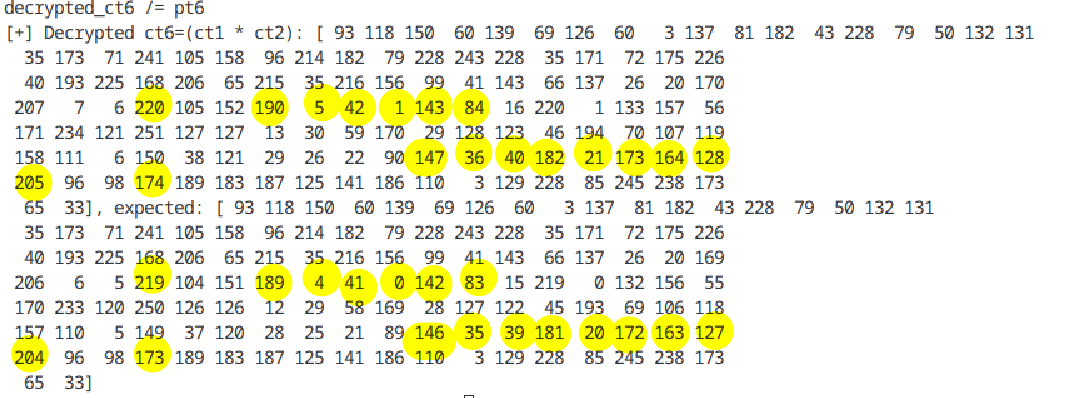
\includegraphics[width=0.6\textwidth]{errored_decryption.png} 
            \caption{Decryption error: example1} 
            \label{fig:errored_dec1}
      \end{figure}

      \begin{figure}[htp] 
            \centering
            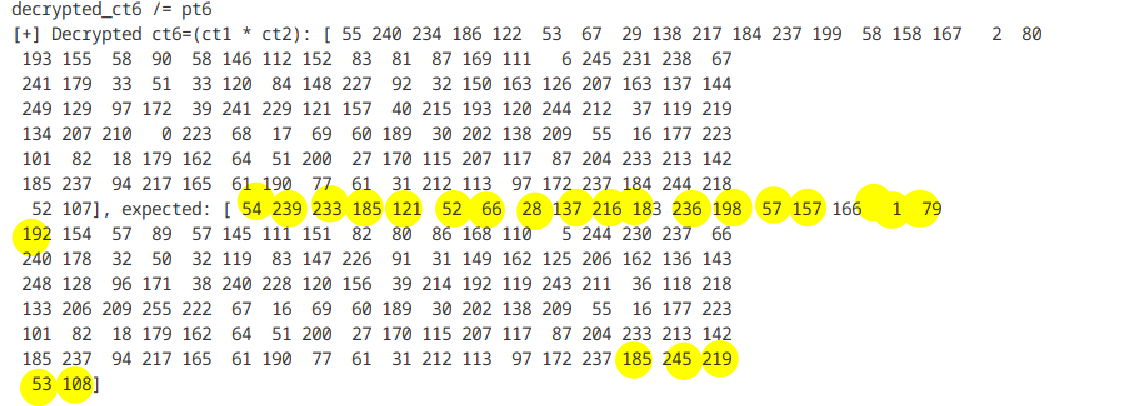
\includegraphics[width=0.6\textwidth]{errored_decryption2.png}
            \caption{Decryption error: example2}
            \label{fig:errored_dec2} 
      \end{figure}

      After some digging the rounding errors might come from the fact that \textit{rlwe\_he\_scheme\_updated.polymul()}
      implementation calculates the final value of multiplication thorough a final modulus
      and np.int64\(\) function.

      The model also fails to work with parameter\_set C due to fact that the cypher text modulo Q=64 is greater that \textit{np.int64\(\)}
      signed implementation of the python model. The might be a similar issue with running decryption algorithm with relinearization\_ver2
      even for Parameter set A. But, relinearization version1 work without issue for the same set.

      Finally, running parameter set B in python is out of question, as Q=512.

    \subsection{Encryption}

    For every message(m) one has to calculate: 
    $$
    c_t = \left( \left[ (pk0 \cdot u + e_1 + \Delta \cdot m) \right]_{R_q} ,
                 \left[ (pk1 \cdot u + e_2) \right]_{R_q} \right)  \in {R_q}\times {R_q}
    $$
    


    \section{Design challenge part1}

    \begin{figure}[htp] 
      \centering
      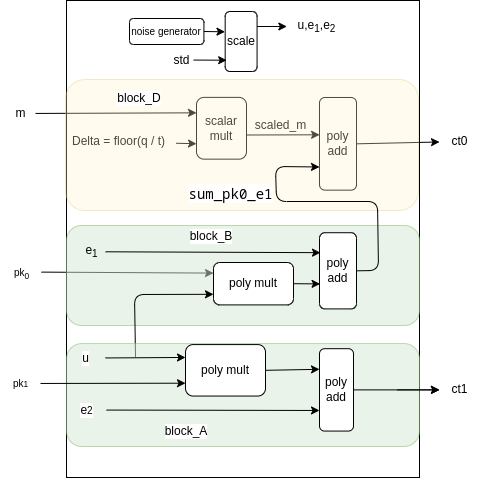
\includegraphics[width=0.6\textwidth]{FV12_encryption.png}
      \caption{System Architecture}
      \label{fig:sysarch} 
    \end{figure}

    \subsection{Analysis}
    From the given use case, we know public key tuple [pk1, pk0] is pre-computed at the host once at the beginning and is used all encryptions.

    for every **m**,
    - sample: r1,r2: normal distribution in R
              u : binary, uniform distribution sample from R
    - $block\_A$  and $block\_B$ operation is independent of $Block\_D$, provided **u** is saved for use in $block\_B$
    - Since q and t are constant $\Delta=\lfloor q/t \rfloor$ is also constant and can be expressed as a power of 2. Hence, scaling is just a left-shift operation on the individual fields of incoming message vector m. 
    
    In our particular case i.e. for parameter sets A and B, m is left shifts of 24 and 448 respectively. 
    It is good to note that even after scaling, field elements of '$scaled\_m$' is never greater than 'q'. So no overflows occur after scaling of field values and can still be represented in 'log2(q)' bits. In our case, it is 32 and 512 bit for parameter sets A and B respectively.
    
    In summary, reducing the latency of encryption is constrained to calculation of one **$poly\_add$** function.
    

    \section{Design challenge part2}
    This part zooms into implementation of $z = pk0 \cdot u$ part of the encrption algorithm. It gives us some idea of the complexity of polynomial
    multiplication even though one of the parameters \textit{u} is just one-bit wide.

    So the hardware needs to do polynomial multiplication of $u \in R_2$ with  $p \in R_q$ to produce a result  $z \in R_q$.
    The fields in/out through an AXI stream interface. 

    \section{Algorithm}
    Polynomial multiplication can be seen as circular convolution coeffcients of the two polynomials. 
    Say N=4, two polynomials  A(x) and B(x) are to be multiplied, the final result $C(x)$ is given as below.

    \begin{align}
      f(x) \ast g(x) &= \sum_{k=0}^{N-1} f(k) \cdot g((n-k) \mod N) \\
      A(x) &= a_0 + a_1x + a_2x^2 + a_3x^3 \\
      B(x) &= b_0 + b_1x + b_2x^2 + b_3x^3 \\
      C(x) = P(x) \times Q(x) &= c_0 + c_1x + c_2x^2 + c_3x^3 + c_4x^4 + c_5x^5 + c_6x^6 \\
      C(x) &= c_0 + c_1x + c_2x^2 + c_3x^3 - c_4 - c_5x - c_6x^2\ \ \   subsituting\ \ \ X^4 = -1 
    \end{align}

    Where,
    \begin{align}
      c_0 &= a_0 \cdot b_0 \\
      c_1 &= a_0 \cdot b_1 + a_1 \cdot b_0 \\
      c_2 &= a_0 \cdot b_2 + a_1 \cdot b_1 + a_2 \cdot b_0 \\
      c_3 &= a_0 \cdot b_3 + a_1 \cdot b_2 + a_2 \cdot b_1 + a_3 \cdot b_0 \\
      c_4 &= a_1 \cdot b_3 + a_2 \cdot b_2 + a_3 \cdot b_1 \\
      c_5 &= a_2 \cdot b_3 + a_3 \cdot b_2 \\
      c_6 &= a_3 \cdot b_3 \\
    \end{align} 
    
    \begin{align}
      C(x) &= (c_0-c_4) + (c_1- c_5)x + (c_2- c_6)x^2 + c_3x^3  \\
      C(x) &= s_0 + s_1x + s_2x^2 + s_3x^3  \\
      s_0 &= (a_0 \cdot b_0 - a_1 \cdot b_3 - a_2 \cdot b_2 - a_3 \cdot b_1 )\ mod Q\\
      s_1 &= (a_0 \cdot b_1 + a_1 \cdot b_0 - a_2 \cdot b_3 - a_3 \cdot b_2 )\ mod Q\\
      s_2 &= (a_0 \cdot b_2 + a_1 \cdot b_1 + a_2 \cdot b_0 - a_3 \cdot b_3 )\ mod Q\\
      s_3 &= (a_0 \cdot b_3 + a_1 \cdot b_2 + a_2 \cdot b_1 + a_3 \cdot b_0 )\ mod Q\\
    \end{align} 
    
    To realise the implementation in hardware, we set N partial product calulators (pprod). Each pprod, starts one clock cycle
    after the previous one and continues to calculate partial product for N clock cycles. Pictorially, it can be shown as in figure \ref{fig:multiplier}. 
    
    pProd0 is active from clk0 to clk3, pProd1 is active from clk1 to clk4, and so on. 
    The final results which are C(0),C(1),C(2),C(3), are read out start clk4,clk5, clk6 and clk7 respectively.

    \begin{figure}[htp] 
      \centering
      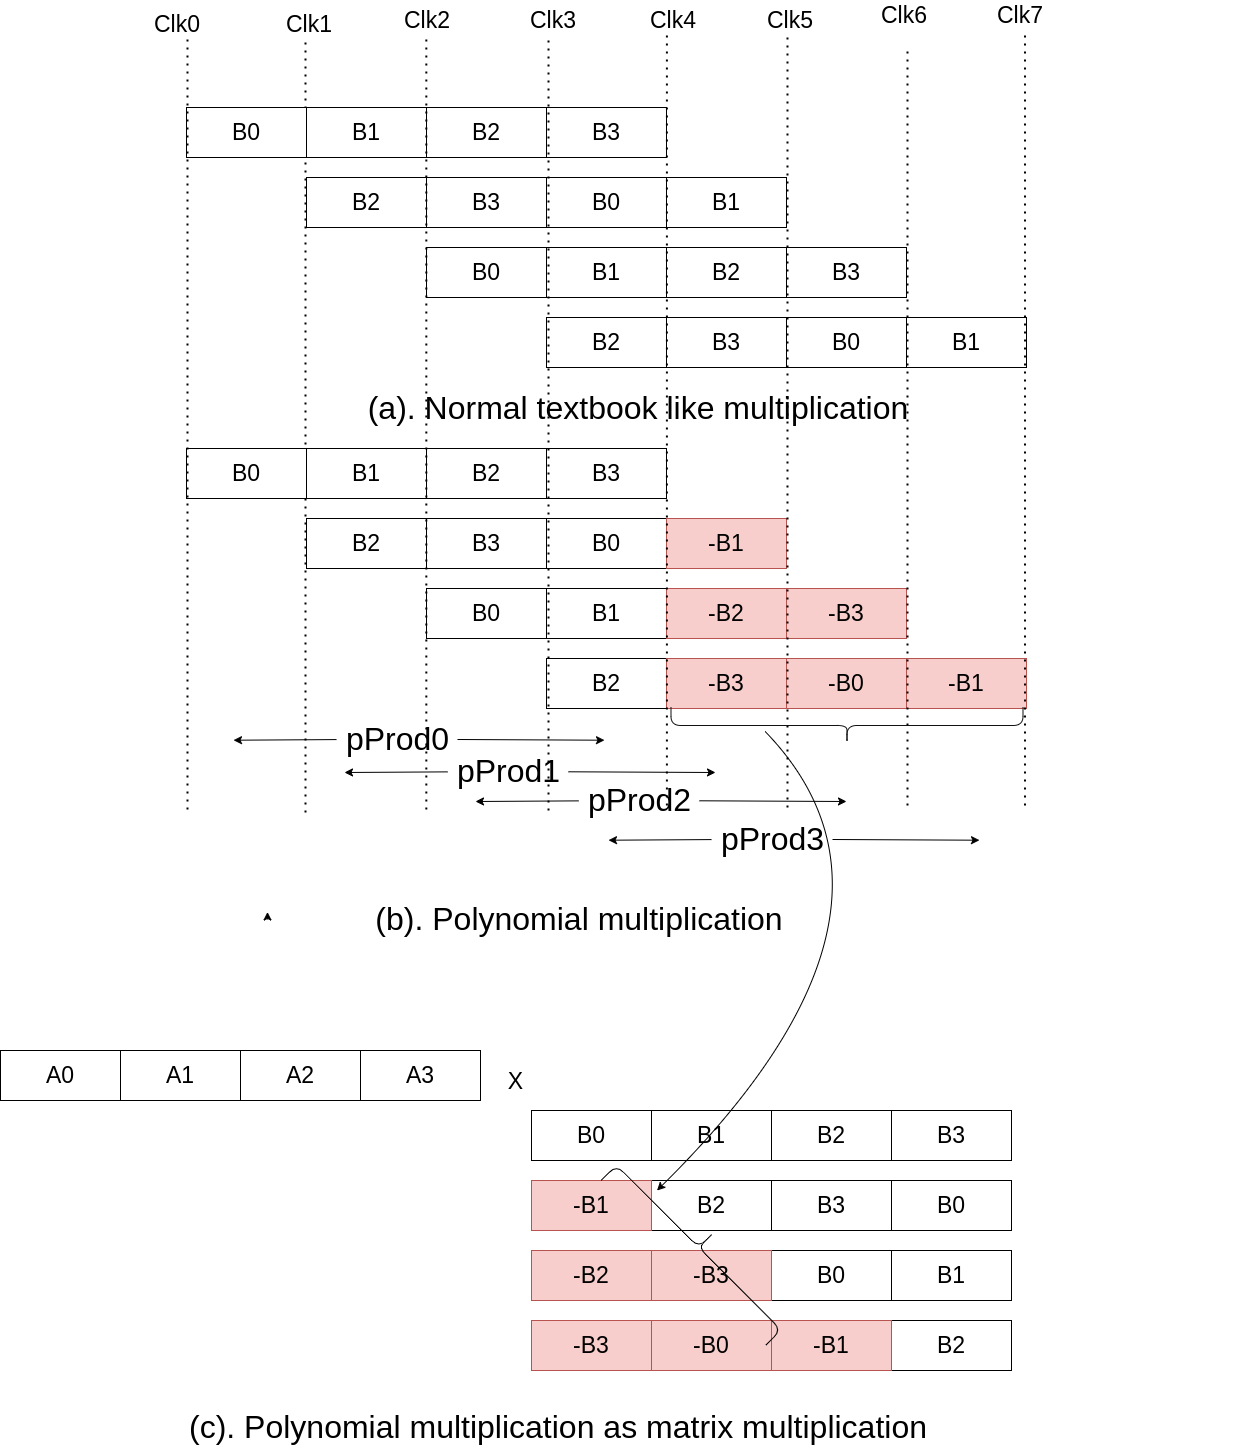
\includegraphics[width=0.6\textwidth]{multiplier_func.png}
      \caption{Multiplier dataflow}
      \label{fig:multiplier} 
    \end{figure}

    Figure \ref{fig:multiplier}.c show calculate C(x) through matrix multiplication. The structure of the matrix is similar to circular 
    convolution matrix except for the sign changes that occurs due to polynomial division.

    In summary, it can be seen serial polynomial multiplication happens in N clock cycles. In order to achieve non-stop streaming operation, two such
    multipliers are instantiated as shown in \ref{ref:multiplier_top} each operating on alternate packets.

    \begin{figure}[htp] 
      \centering
      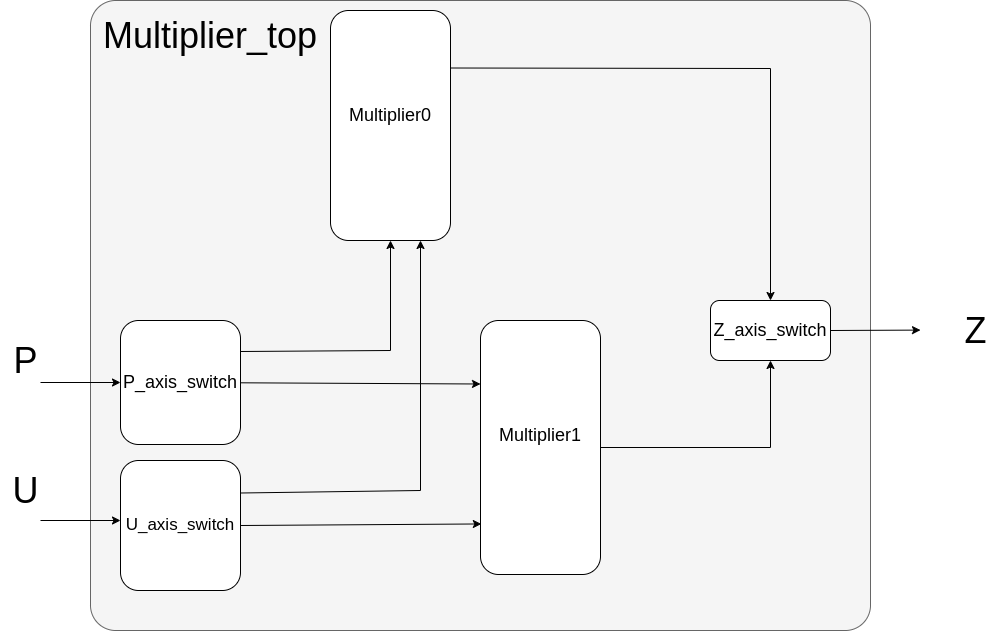
\includegraphics[width=0.6\textwidth]{multiplier_top.png}
      \caption{Multiplier top instance}
      \label{fig:multiplier_top} 
    \end{figure}

    \subsection{Simulation}
    The simulation environment is abysmally simplistic, in order meet the task completion deadline. Ideally, cocotb would have
    been used for faster checking. But that would have meant mandatory use of cocotb for even simple code sanity check. 

    The code in \textit{tb\_multiplier.sv} instantiates \textit{multiplier\_top} by default. This instantiates two multipliers 
    and streams 3 packets back-to-back. To test only the single multipler one can just change the instance name to \textit{multiplier} 
    and comment extra packets being sent. 

    \section{What if...more time was given?}

    As the saying goes with if's and buts one can build castles in the air. But being pragmatic, these are the top priorities in the to do list
    \begin{itemize}
      \item Spend time in reading and understanding  in detail basic algorithms, 
    \end{itemize}
    % \section{Hello World!} % creates a section
    
    % \textbf{Hello World!} Today I am learning \LaTeX. %notice how the command will end at the first non-alphabet charecter such as the . after \LaTeX
    %  \LaTeX{} is a great program for writing math. I can write in line math such as $a^2+b^2=c^2$ %$ tells LaTexX to compile as math
    %  . I can also give equations their own space: 
    % \begin{equation} % Creates an equation environment and is compiled as math
    % \gamma^2+\theta^2=\omega^2
    % \end{equation}
    % If I do not leave any blank lines \LaTeX{} will continue  this text without making it into a new paragraph.  Notice how there was no indentation in the text after equation (1).  
    % Also notice how even though I hit enter after that sentence and here $\downarrow$
    %  \LaTeX{} formats the sentence without any break.  Also   look  how      it   doesn't     matter          how    many  spaces     I put     between       my    words.
    
    % For a new paragraph I can leave a blank space in my code. 

\end{document} % This is the end of the document
